
\section{Overview}
\label{sec:overview}
\sysname is a smartphone-based blood glucose level tracking system that \emph{(i)} non-intrusively collects important external impacting factors and conducts feature engineering, \emph{(ii)} efficiently trains a personalized blood glucose level model, and \emph{(iii)} timely reminds users of abnormal blood glucose levels.
\figref{fig:architecture} shows the architecture of \sysname, which consists of three modules.

\begin{figure}[h]
  \centering
  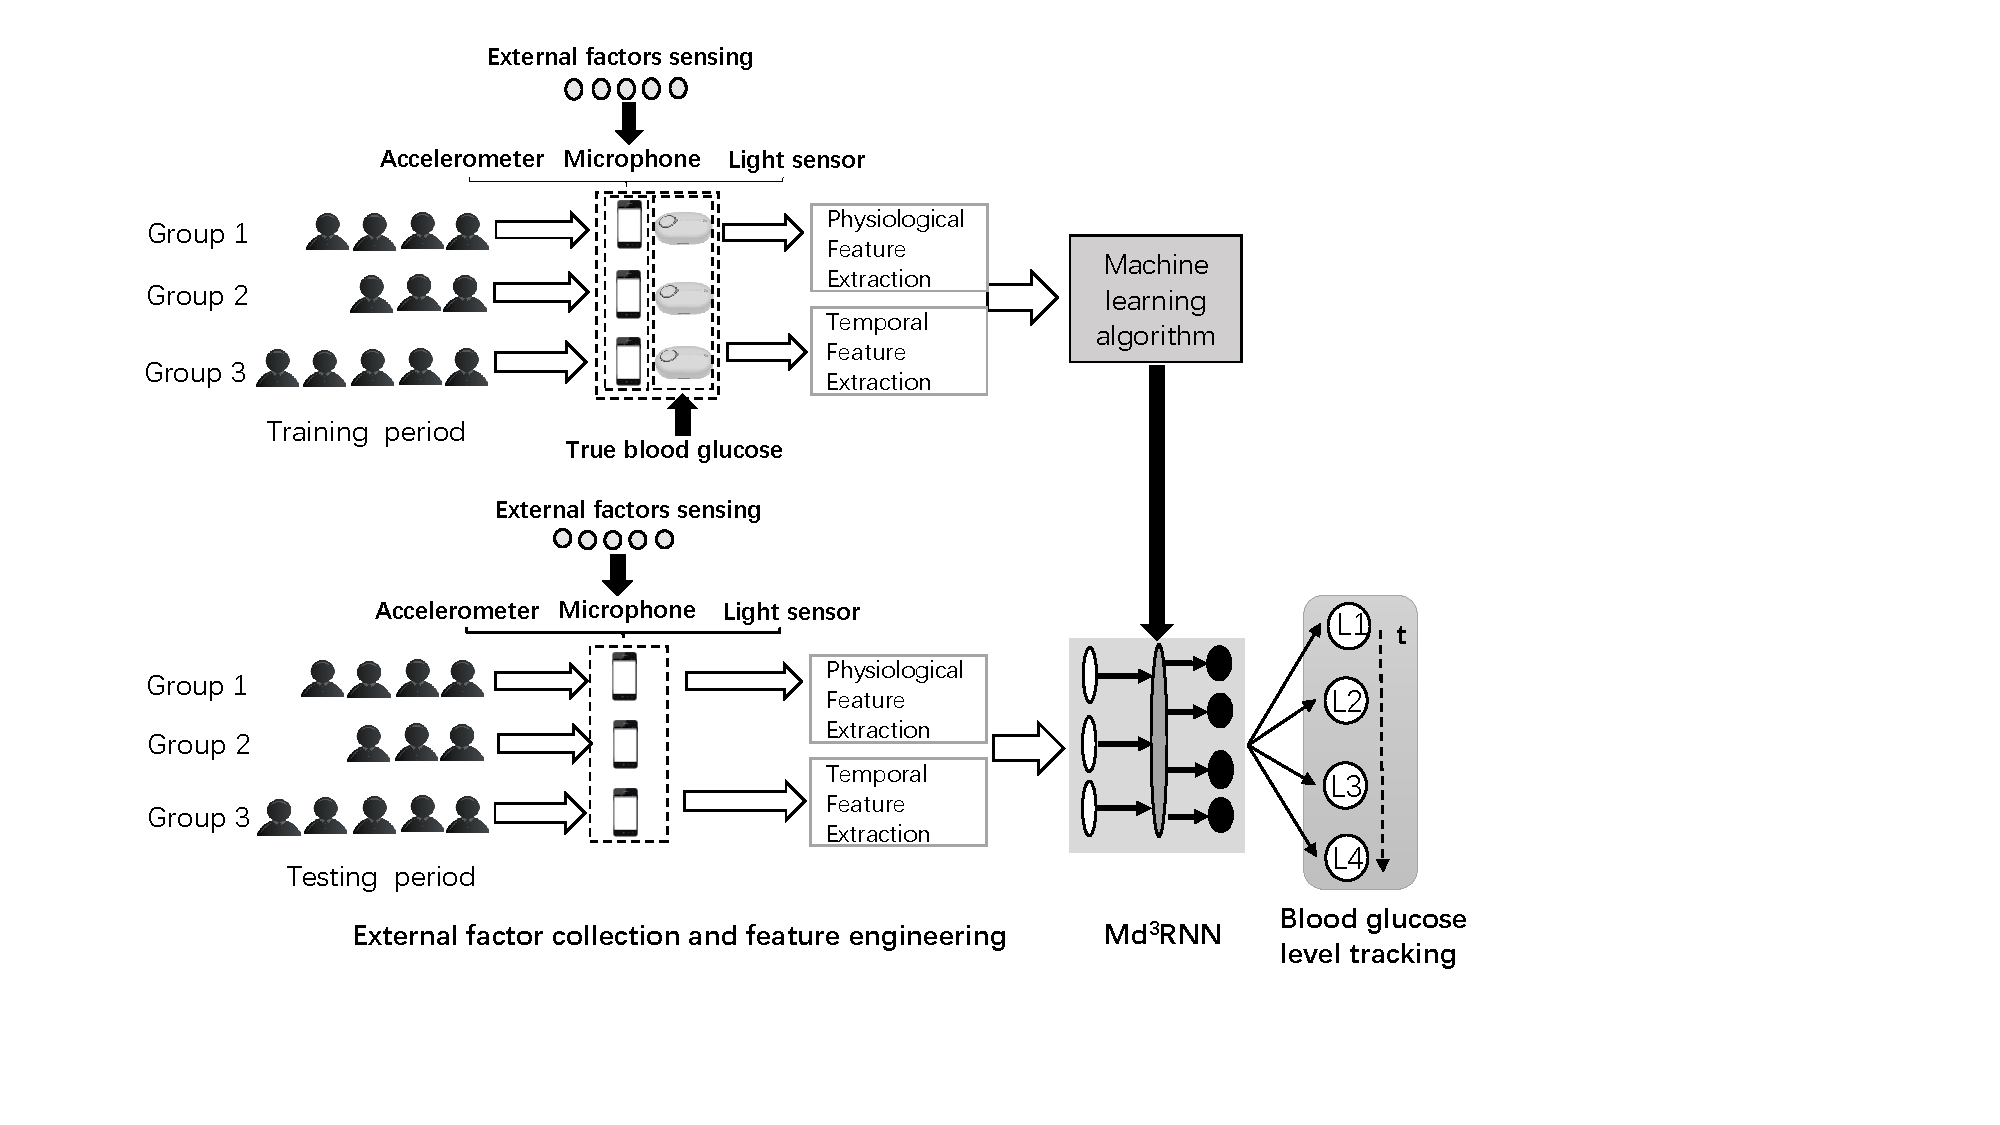
\includegraphics[width=0.8\columnwidth]{./img/System_Arch2.pdf}
  \caption{Architecture of \sysname.}
  \label{fig:architecture}
\end{figure}

The \textbf{external factor collection and feature engineering} module records external factors that are important to infer blood glucose levels.
A user records daily meal, drug and insulin intake.
Meanwhile, \sysname automatically measures physical activities and sleep quality via embedded sensors (\ie accelerometer, microphone and light sensor).
After collecting data from multiple users, \sysname conducts feature engineering from physiological and temporal perspectives, and feeds them into \textbf{\modelname}, a multi-division deep learning framework specific designed for blood glucose inference.
\modelname first learns feature representations from users in the same group (non-diabetic, Type I and Type II diabetic), and then adopts a deep RNN layer to learn a general blood glucose level model on the dataset of all users.
Finally, it outputs a personalized blood glucose level model for each individual via a personality layer. 
The inference results are eventually shown in the \textbf{blood glucose level tracking} module at a fine grained time resolution \rev{(every 3 minutes by default)}.
In \sysname, we consider 4 blood glucose levels as in \tabref{tab:blood_glucose_levels}.

\begin{table}[h]
  \centering
  \caption{Normal and abnormal blood glucose levels~\cite{bib:BGWiKi}.}
  \label{tab:blood_glucose_levels}
  \begin{tabular}{|c|c|c|}
  \hline
  \textbf{Blood Glucose Value (mmol/L)} & \textbf{Glocose Level} & \textbf{Explanation}                      \\ \hline
  (0, 4.4{]}                            & Level 1                & Low blood glucose (hypoglycemia)         \\ \hline
  (4.4, 6.1{]}                          & Level 2                & Normal level of fasting blood glucose      \\ \hline
  (6.1, 7.8{]}                          & Level 3                & Normal level of postprandial blood glucose \\ \hline
  (7.8, $+\infty$)                      & Level 4                & High blood glucose (hyperglycemia)          \\ \hline
  \end{tabular}
\end{table}
